\documentclass[a4paper]{article}
\usepackage[utf8]{inputenc}
\usepackage[a4paper, total={6in, 8in}]{geometry}
\usepackage[english]{babel}
\usepackage{graphicx}
\usepackage[export]{adjustbox}
\usepackage{subcaption}
\usepackage{wrapfig}
\usepackage{array}
\usepackage{multirow}
\usepackage{makecell}
\usepackage{hhline}
\usepackage{lipsum}
\usepackage[pdftex,dvipsnames,table]{xcolor}
\usepackage{xcolor}
\usepackage{graphicx}
\usepackage{float}
\usepackage{longtable}
\usepackage[bottom]{footmisc}

\usepackage{hyperref}

% code package
\usepackage{listings}

% comment package
\usepackage{comment}

% ToDo package and config
\usepackage{xargs}
\usepackage[colorinlistoftodos,prependcaption,textsize=tiny]{todonotes}
\newcommandx{\mytodo}[2][1=]{\todo[linecolor=red,backgroundcolor=red!25,bordercolor=red,#1]{#2}}
\usepackage{marginnote}
\renewcommand{\marginpar}{\marginnote}

% VU colors
\definecolor{vu-black}{HTML}{000000}
\definecolor{vu-white}{HTML}{ffffff}
\definecolor{vu-grey-80}{HTML}{333333}
\definecolor{vu-grey-50}{HTML}{e1e1e1}
\definecolor{vu-blue}{HTML}{007ab9}

% vars
\newcommand{\arraystrechlength}{1.5}

\begin{document}

%title
\begin{center}
\vspace{1mm}

\includegraphics[height=18mm]{figs/VUlogo.png}

\vspace*{1.5cm}

\rule{.9\linewidth}{.6pt}\\[0.4cm]
{\huge \bfseries Software Testing 2020 \par}
\vspace{0.2cm}
{\large \bfseries \textit{Assignment PROJECT: Heart Monitor}\par}
{\large \bfseries \textit{Software Requirements Specification}\par}\vspace{0.4cm}
\rule{.9\linewidth}{.6pt}\\[1.5cm]


\vspace*{2mm}


{\large
    \begin{tabular}{rl}
    \textbf{Group:} & 11 - Korean Air \\ \\
    \textbf{Members:} & Markus Funke (2644722)  \\
                & Wouter Kok (2639768) \\
                & Sven Preng (2614131) \\
                & Pjotr Scholtze (2612369)  \\ \\
    \textbf{Master program:} & Computer Science - SEG
  \end{tabular}%
}


\vspace*{5cm}

\today\\[4cm] % Date
\thispagestyle{empty}
\end{center}



\tableofcontents
\thispagestyle{empty}
\pagenumbering{arabic}
\clearpage


\renewcommand{\arraystretch}{1.5}


%%%%
% Introduction
%%%%
\section{Introduction}
\label{sec:intro}

\subsection{Purpose}
\begin{comment}
Purpose of this specific SRS and mention the audience for the SRS. In our case this would be probably a) the developer (we), b) the testing group (other students), c) the customer (teacher).
\end{comment}
This Software Requirements Specification (SRS) is regarding the Heart Beat Monitor Simulation Software \textbf{HB-Sim2020} that is to be developed during the Software Testing course at the VU (2019-2020). The document is intended for future developers, testers, the product owner and other stakeholders.

\subsection{Scope}
\begin{comment}
\begin{enumerate}
    \item Identify SW products by name (Heart Monitor XL)
    \item Explain what the SW products will, and will not do (will trigger alarms, will not be connected to physical sensors)
    \item Describe the app of the SW being specific (benefits, objectives, goals)
\end{enumerate}
\end{comment}

The  Heart Beat Monitor Simulation Software is to be developed as part of the PROJ assignment of the Software Testing course. The main purpose of the software is to be  tested after development to discuss the possible bugs for educational purposes. The software will run a simulation of a generic heartbeat monitor used in a medical facility. The heartbeat monitor should be able to notify the medical team of any anomalies in the oxygen levels, heart beat and blood pressure as well as give a constant update on these current values via a command line interface. Since this software should simulate a heartbeat monitor, it is not connected to any actual sensors and thus will receive it's input through a test file. 

\subsection{Definitions, acronyms, and abbreviations}
\begin{itemize}
    \item HB-Sim2020 - Heart Beat Monitor Simulation Software
    \item SRS - Software Requirements Specification
    \item BPM - Beats Per Minute
    \item CSV - Comma-separated values
    \item CLI - Command Line Interface
    \item QAS - Quality Attribute Scenario
    \item mmHg - millimeter of mercury
    \item HR - Heart Rate
    \item BP - Blood Pressure
\end{itemize}

\subsection{Technologies to be used}
To adhere to the standards for the PROJ assignment, the software will be written in a recent version of python (3.7.7) while using minimal external libraries in order to reduce possible bugs that might be introduced by such libraries. A comprehensive overview of all relevant and used technologies/libararies can be found in section \ref{appendix:python-libs}. 

\subsection{Overview}
The SRS is organized as follows. Section \ref{sec:intro} introduces the document, section \ref{sec:overall} describes the general factors that affect the product and its requirements. It provides background for the actual requirements which are defined in section \ref{sec:non-func-req} and \ref{sec:func-req}. The non-functional requirements describes \textit{how} the system \textit{should} work. The functional requirements examine the specific behavior of the \textit{HB-Sim2020} system and what the system is supposed to \textit{do}.


\clearpage
%%%%
% Overall description
%%%%
\section{Overall description}
\label{sec:overall}
\begin{comment}
Should describe the general factors that affect the product and its requirements. \textbf{This section does NOT state specific requirements}. Instead, it provides background for those requ. which are defined in section 3.

Use case Model Diagram or other diagrams (like ER-diagram or architecture overview). 
\end{comment}

\subsection{Product perspective}
\begin{comment}
Put the product into perspective with other realted products. If the product is independent and self-contained (in our case YES), it should be so stated here.

A block diagram could show the major components of the larger system and connections. (I think we do not have those?)
\end{comment}
The implemented system \textit{HB-Sim2020} can be defined as virtual implementation of an actual hardware based heart rate monitor. Since a hardware monitor is connected to actual a) pulse-, b) blood-pressure-, and c) oxygen-sensors, the virtual implementation needs to work without any real sensor connections. Figure \ref{fig:overview-real} and figure \ref{fig:overview-virtual} distinguish the two different approaches in a visual manner. While the real world environment uses an actual wave analyzer to display the current values, the virtual environment uses a comma-separated-value (CSV) file to simulate incoming sensor data and prints all values and messages to a Command Line Interface (CLI) in a text based manner. The following sections all refer to the virtual environment as in figure \ref{fig:overview-virtual}.


\begin{figure}[H]
\centering
    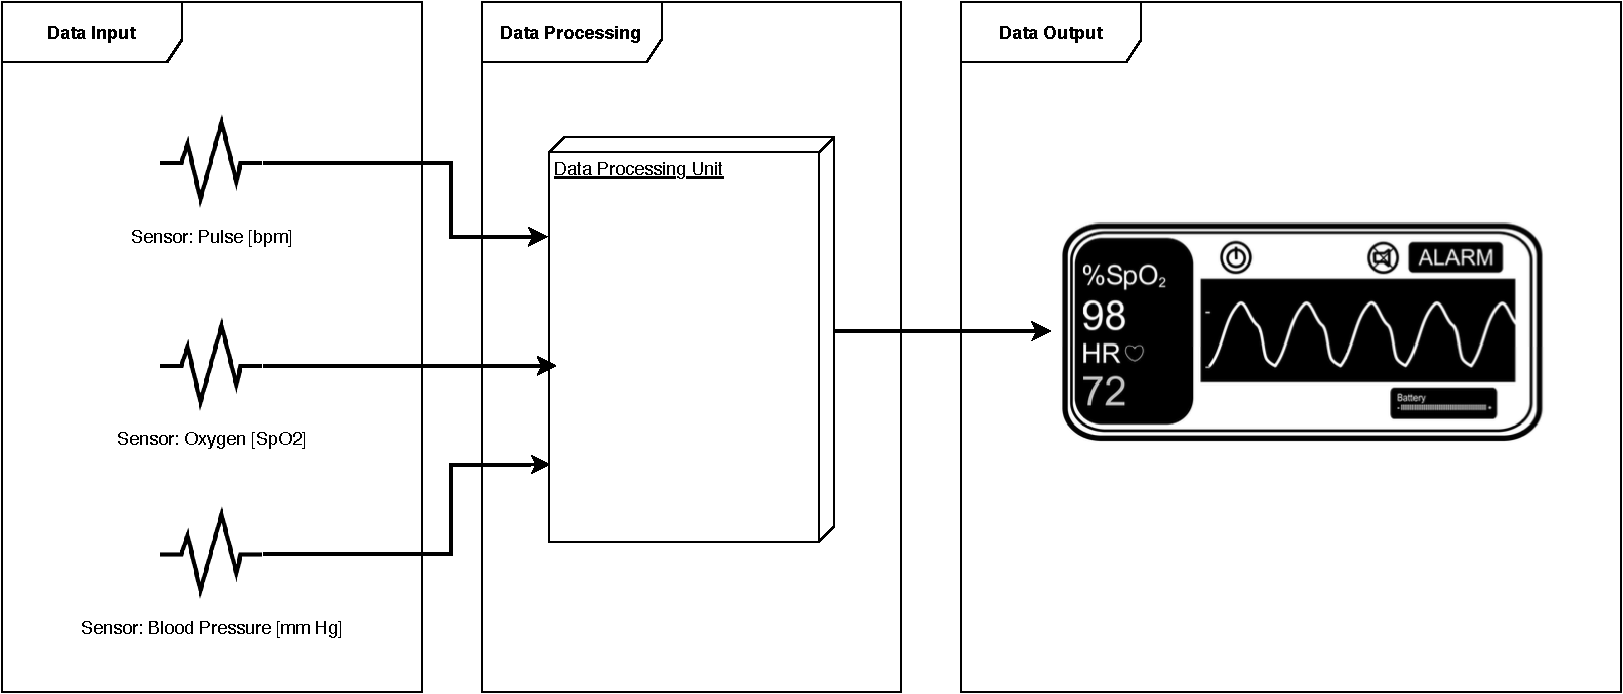
\includegraphics[scale=0.4]{ST_2019_Project_ Requirements/figs/overview_real.pdf}
    \caption{Heart Rate Monitor - real world environment (image: \cite{b1})}
    \label{fig:overview-real}
\end{figure}

\begin{figure}[H]
\centering
    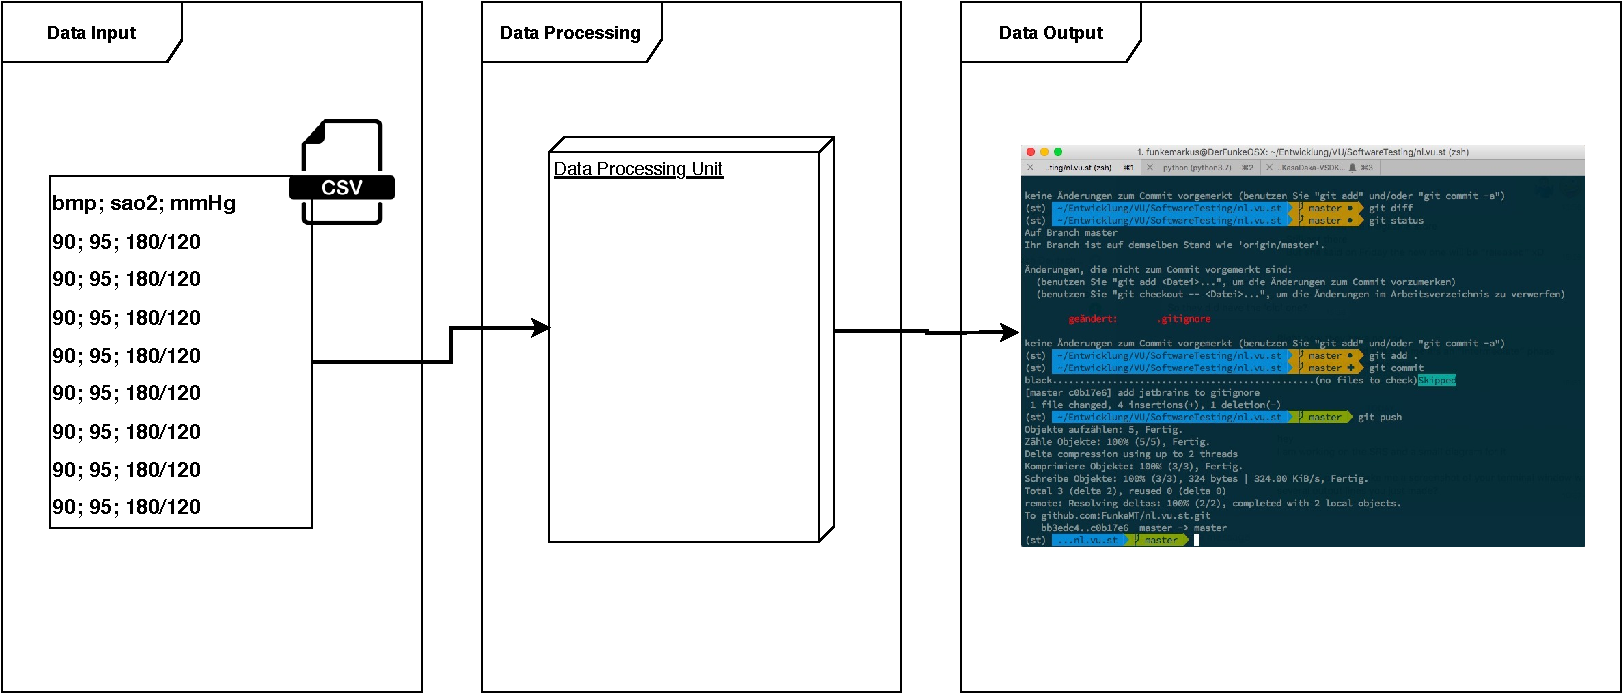
\includegraphics[scale=0.40]{ST_2019_Project_ Requirements/figs/overview_virtual.pdf}
    \caption{Heart Rate Monitor - virtual environment}
    \label{fig:overview-virtual}
\end{figure}

\subsubsection{System interfaces}
The system collects data from a CSV file exclusively which simulates real sensor data. The necessary file structure and requirements are described in section \ref{sec:data-input:csv-file}. Beyond, the system is connected to the file system for logging. If the disk is full or if the user has no write access, the program will not stop; it will inform the user that it cannot write to disk and will still continue to operate. The CSV file is the only interface which is connected to the system.

\subsubsection{User interfaces}
The user interface is provided as CLI prompt. The CLI offers the option to specify the CSV path at program start. After initialisation, no further user inputs are available and valid. The program works autonomous and switches to the data processing mode. Whilst the program is in this mode, the CLI presents the processed data and various information. Detailed information about the user interface is explained in section SR\#\ref{ftr:ui}

\subsubsection{Operations}
It is required that the user provides a CSV file for the program. The CSV file should have a header with the fields as denoted in \ref{ftr:csv-file}, every other row should contain unsigned integer values with a data snapshot. Every row after the heading represents a snapshot of data, the program interprets every row as a unit of time defined in \ref{sec:data-input:csv-file}.

% Defines the normal and special operations required by the user to use our program. E.g. enter patient age, weight

\clearpage
\subsection{Medical Terms}
Since the system deals with several medical units and medical terms, the following section provides a brief overview of the different units in use.

\subsubsection{Heart Rate (pulse)}
\begin{table}[H]
{\renewcommand{\arraystretch}{\arraystrechlength}
\begin{tabular}{ | >{\columncolor{vu-blue}\color{vu-white}}m{70pt} | >{\columncolor{vu-grey-50}}m{80pt} | p{238pt} | } 
\hline
Heart Rate \newline (pulse) & Abbreviation & $HR$  \\ 
\hline
                          & Unit   & \texttt{bpm} - beats per minute                   \\ 
\hline
                          & Value range  & $0bpm ... 230bpm$ (exclusive)                        \\ 
\hline
                          & Description  & 
                          "Heart rate is the speed of the heartbeat measured by the number of contractions (beats) of the heart per minute (bpm). The heart rate can vary according to the body's physical needs, including the need to absorb oxygen and excrete carbon dioxide. It is usually equal or close to the pulse measured at any peripheral point. Activities that can provoke change include physical exercise, sleep, anxiety, stress, illness, and ingestion of drugs."\cite{b2}
                          \newline\newline
                          Heart Rate and Pulse are used interchangeable throughout the document. Pulse is used in the application.
                          \\ 

\hline
\end{tabular}
}
\caption{Heart rate}
\label{table:heart-rate}
\end{table}

\subsubsection{Oxygen}
\begin{table}[H]
{\renewcommand{\arraystretch}{\arraystrechlength}
\begin{tabular}{ | >{\columncolor{vu-blue}\color{vu-white}}m{70pt} | >{\columncolor{vu-grey-50}}m{80pt} | p{238pt} | } 
\hline
Oxygen                & Abbreviation & $SpO_{2}$  \\ 
\hline
                          & Unit   & $\%$ - percent                   \\ 
\hline
                          & Value range  & $0\% ... 100\%$                        \\ 
\hline
                          & Description  & 
                          "Oxygen saturation is the fraction of oxygen-saturated hemoglobin relative to total hemoglobin (unsaturated + saturated) in the blood. The human body requires and regulates a very precise and specific balance of oxygen in the blood. Normal arterial blood oxygen saturation levels in humans are 95–100 percent."\cite{b3}
                          \\ 

\hline
\end{tabular}
}
\caption{Oxygen}
\label{table:oxygen}
\end{table}

\subsubsection{Blood Pressure}
\begin{table}[H]
{\renewcommand{\arraystretch}{\arraystrechlength}
\begin{tabular}{ | >{\columncolor{vu-blue}\color{vu-white}}m{70pt} | >{\columncolor{vu-grey-50}}m{80pt} | p{238pt} | } 
\hline
Blood pressure                & Abbreviation & $BP$  \\ 
\hline
                          & Unit   & $mmHg$ - millimeter of mercury                   \\ 
\hline
                          & Value range  & $0/0mmHg ... 300/300mmHg$                        \\ 
\hline
                          & Description  & 
                          "Blood pressure (BP) is the pressure of circulating blood on the walls of blood vessels. Most of this pressure is due to work done by the heart by pumping blood through the circulatory system. Used without further specification, "blood pressure" usually refers to the pressure in large arteries of the systemic circulation. Blood pressure is usually expressed in terms of the \textbf{systolic pressure} (maximum during one heartbeat) over \textbf{diastolic pressure} (minimum in between two heartbeats) and is measured in millimeters of mercury (mmHg), above the surrounding atmospheric pressure."\cite{b4}
                          \\ 

\hline
\end{tabular}
}
\caption{Blood pressure}
\label{table:blood-pressure}
\end{table}


\clearpage
\subsection{Product functions}
\begin{comment}
Provide a summary of the major functions (measure data, trigger alarms, bla bla). 
Organize the functions in a way that makes the list of functions understandable for anyone who is reading the doc for the first time.
Diagrams can be used to show the different functions and their relationships.
We could offer here a diagram for an example use case when an alarm is triggered, etc.?
\end{comment}

This section examines the product features in a high level manner. Detailed and traceable functional requirements are described and examined in the actual requirements section \ref{sec:func-req}. Functions can be grouped into three different groups, i.e. i) data input, ii) data processing, and iii) data output. The groups contain multiple sub-functions.

\subsubsection{Data input}
\begin{table}[H]
{\renewcommand{\arraystretch}{\arraystrechlength}
\begin{tabular}{ | >{\columncolor{vu-blue}\color{vu-white}}m{70pt} | >{\columncolor{vu-grey-50}}m{80pt} | p{238pt} | } 
\hline
Data input              & CLI & CSV location can be specified by a command-line argument at program start.  \\ 
\hline
                        &    & CLI provides a \textit{help} menu. \\ 
\hline
                        &  CSV  & CSV file simulates the sensor data. \\ 
\hline                          
                        &    & The CSV file contains all necessary sensors (blood pressure, heart rate, oxygen) and their possible circumstances (no data, corrupted data, etc.) \\ 
\hline
\end{tabular}
}
\caption{Functions - data input}
\label{table:func-data-input}
\end{table}

\subsubsection{Data processing}
\begin{table}[H]
{\renewcommand{\arraystretch}{\arraystrechlength}
\begin{tabular}{ | >{\columncolor{vu-blue}\color{vu-white}}m{70pt} | >{\columncolor{vu-grey-50}}m{80pt} | p{238pt} | } 
\hline
Data processing         & validation & Input values will be validated against specific rules (i.e. numeric values, strings, etc.)  \\ 
\hline
                        & error handling   & Corrupted incoming values will be handled without terminating the program. \\ 
\hline
                        & blood pressure   & Processing and evaluation. \\ 
\hline
                        & oxygen   & Processing and evaluation. \\ 
\hline
                        & heart rate   & Processing and evaluation. \\ 
\hline
                        & statistic   & A statistic keeps track of all processed values. \\ 
\hline
\end{tabular}
}
\caption{Functions - data processing}
\label{table:func-data-processing}
\end{table}

\subsubsection{Data output}
\begin{table}[H]
{\renewcommand{\arraystretch}{\arraystrechlength}
\begin{tabular}{ | >{\columncolor{vu-blue}\color{vu-white}}m{70pt} | >{\columncolor{vu-grey-50}}m{80pt} | p{238pt} | } 
\hline
Data output             & CLI & All messages will be printed to the CLI.  \\ 
\hline
                        &    & The messages will be formatted in a proper manner such that the messages can be read easily.  \\ 
\hline
                        & status messages & Status messages contain the \textit{status, value, unit} of oxygen, heart rate, and blood pressure.  \\ 
\hline                         
                        &  statistic  & A statistic of all processed values will be displayed if the program ends or terminates.  \\ 
\hline
\end{tabular}
}
\caption{Functions - data output}
\label{table:func-data-output}
\end{table}


\begin{comment}
\subsubsection{Data input}
\begin{table}[H]
{\renewcommand{\arraystretch}{\arraystrechlength}
\begin{tabular}{ | >{\columncolor{vu-blue}\color{vu-white}}m{70pt} | >{\columncolor{vu-grey-50}}m{80pt} | p{238pt} | } 
\hline
Data input              & CLI & CSV location can be specified by command-line argument at program start.  \\ 
\hline
                        &    & CLI provides a \textit{help} menu. \\ 
\hline
                        &  CSV  & CSV file simulates the sensor data. \\ 
\hline                          
                        &    & First-line contains the order of values (heading). This means that the file is resilient against different orders. \\ 
\hline
                          &    & File should contain values for heart rate, oxygen and blood pressure. Blood pressure contains out of "systolic" and "diastolic". \\ 
\hline
\end{tabular}
}
\caption{Functions - data input}
\label{table:func-data-input}
\end{table}

\subsubsection{Data processing}
\begin{table}[H]
{\renewcommand{\arraystretch}{\arraystrechlength}
\begin{tabular}{ | >{\columncolor{vu-blue}\color{vu-white}}m{70pt} | >{\columncolor{vu-grey-50}}m{80pt} | p{238pt} | } 
\hline
Data processing         & validation & Input values will be validate against specific rules (i.e. numeric values, strings, etc.)  \\ 
\hline
                        & error handling   & Corrupted incoming values will be handled without terminating the program. \\ 
\hline
                        & blood pressure   & Measurement is processed separately. \\ 
\hline
                        &    & Validation against several rules. \\ 
\hline
                        &    & Keeping track of the number of measurements and their status. \\ 
\hline
                        & oxygen   & Measurement is processed separately. \\ 
\hline
                        &    & Validation against several rules. \\ 
\hline
                        &    & Keeping track of the number of measurements and their status. \\ 
\hline
                        & heart rate   & Measurement is processed separately. \\ 
\hline
                        &    & Validation against several rules. \\ 
\hline
                        &    & Keeping track of the number of measurements and their status. \\ 
\hline
                        & statistic   & A statistic keeps track of all processed values. \\ 
\hline
                        &    & The statistic will be displayed at the end of the program. \\ 
\hline
\end{tabular}
}
\caption{Functions - data processing}
\label{table:func-data-processing}
\end{table}

\subsubsection{Data output}
\begin{table}[H]
{\renewcommand{\arraystretch}{\arraystrechlength}
\begin{tabular}{ | >{\columncolor{vu-blue}\color{vu-white}}m{70pt} | >{\columncolor{vu-grey-50}}m{80pt} | p{238pt} | } 
\hline
Data output             & CLI & All messages will be printed to the CLI.  \\ 
\hline
                        &    & The messages will be formatted in a proper manner such that the messages can be read easily.  \\ 
\hline
                        & status messages & Status messages contain the \textit{status} of oxygen, heart rate, and blood pressure.  \\ 
\hline
                        &    & Status messages contain the \textit{value} of oxygen, heart rate, and blood pressure.  \\ 
\hline                          
                        &    & Status messages contain the \textit{unit} of oxygen, heart rate, and blood pressure.  \\ 
\hline                          
                        &  statistic  & A statistic of all processed values will be displayed if the program ends or terminates.  \\ 
\hline
\end{tabular}
}
\caption{Functions - data output}
\label{table:func-data-output}
\end{table}

\begin{table}[H]
{\renewcommand{\arraystretch}{\arraystrechlength}
\begin{tabular}{ | >{\columncolor{vu-blue}\color{vu-white}}m{70pt} | >{\columncolor{vu-grey-50}}m{80pt} | p{238pt} | } 
\hline
Comprehensive features                & ? & bla  \\ 
\hline
                          & ?   & bla \\ 
\hline
\end{tabular}
}
\caption{Functions - comprehensive features}
\label{table:func-comprehensive}
\end{table}
\end{comment}



\subsection{Entity Relation Diagram}
\begin{figure}[H]
\centering
    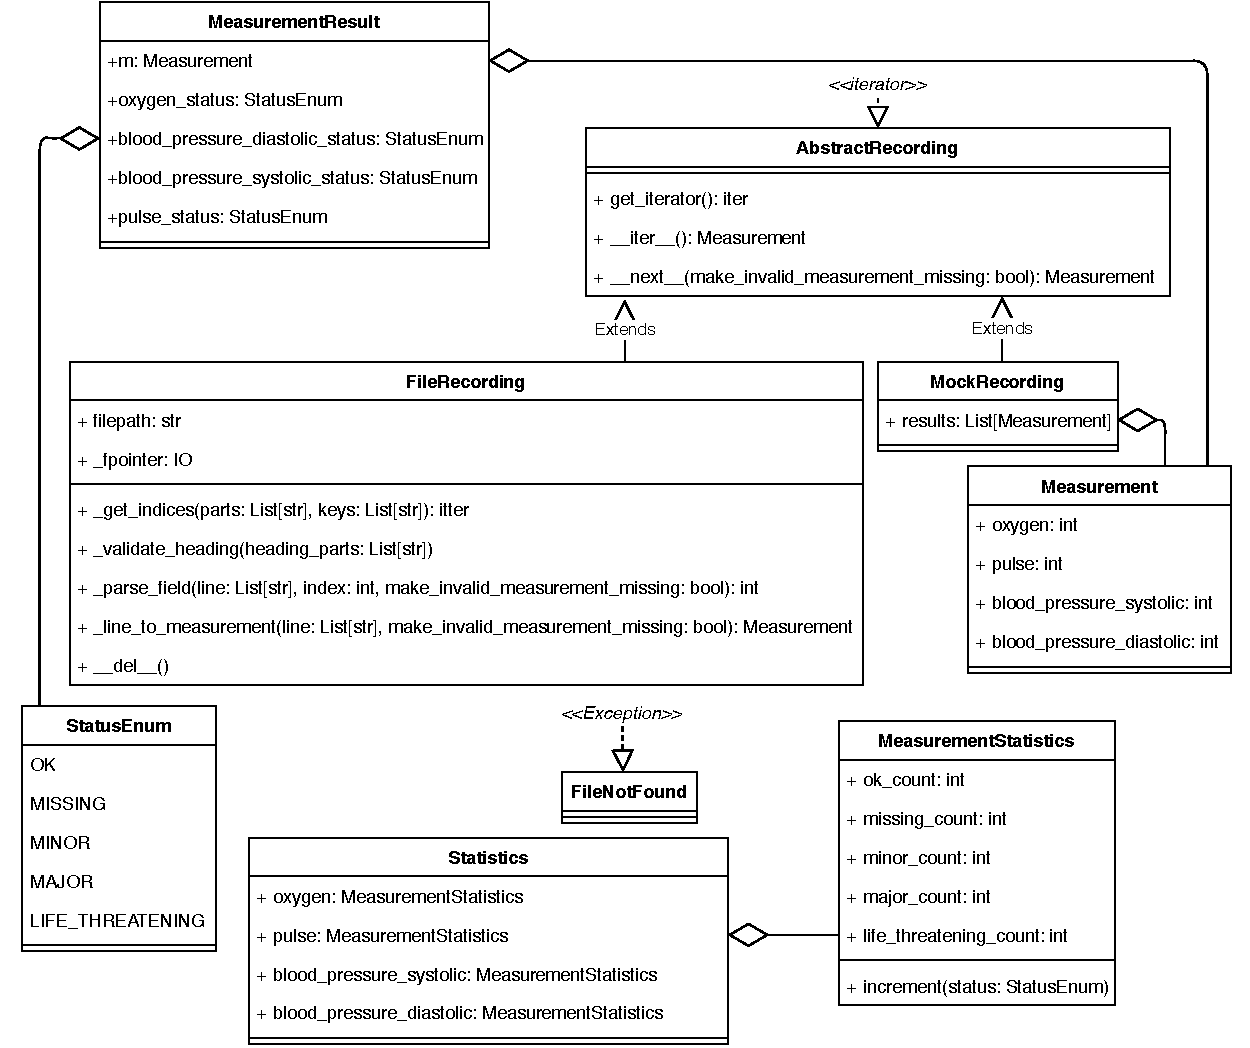
\includegraphics[scale=0.70]{ST_2019_Project_ Requirements/figs/er_diagram.pdf}
    \caption{ER Diagram}
    \label{fig:er-diagram}
\end{figure}


\clearpage
\subsection{Constraints}
\label{sec:constraints}
This section lists restrictions that had to be made due to time and scope constraints.

\begin{enumerate}
    \item The scope of systems the program needs to support are:
    \begin{itemize}
        \item Windows 10 with Linux subsystem version: Linux 4.4.0-18362-Microsoft x86\_64
        \item Windows 10 10.0.18363 Build 18363
        \item Linux Ubuntu 20.04 x64
        \item MacOS 10.13.6
    \end{itemize}
    \item The architecture of the operating system has to be: x64.
    \item The program will be written in Python 3. Other operating systems (version) that are supported by Python but are not listed above are not officially supported by our application.
    \item The program will be written on the assumption that the system has enough RAM available. This is a requirement to run the application, and any hardware that will run our application needs at least 256MB of free ram before the program should be executed. However, the program should not have to check this requirement.
    \item The program does not require any special permissions on the host operating system other then those required to read the intended file from the file system and permission to write if logging is required. However, if writing permissions are not available, the system will omit logging and inform the user.
    \item The program does not check for credentials before running.
    \item The program does not need to check whether the file has been manipulated. 
    \item The program does not need to work with real sensors, a CSV file will simulate the sensors.
    \item The program does not support network paths.
    \item The program does not check the CSV file size or out-of-memory problems. 
    \item For this system we do not have access to actual sensors for the required measurements. For this reason we choose to work with CSV input under the assumption that this file is in the correct format available in SR\#\ref{ftr:csv-file}.
\end{enumerate}

\clearpage
%%%%
% Specific non-functional requirements
%%%%
\section{Specific non-functional requirements}
\label{sec:non-func-req}
The non-functional requirements are expressed as Quality Attribute Scenarios (QAS). The scenarios are defined through a specific source, which triggers the whole scenario and leads into the response measure.

\subsection{Reliability}
\label{qa:reliability}
\textbf{ID: QA-\#\ref{qa:reliability}}
\begin{figure}[H]
\centering
    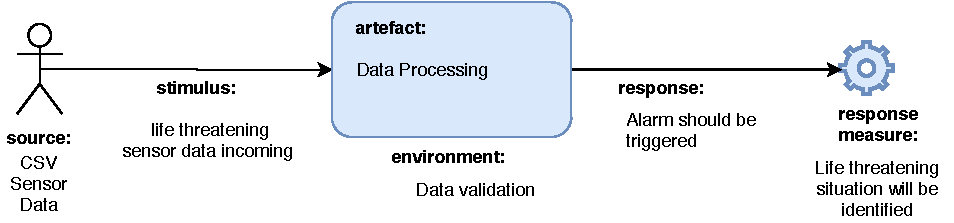
\includegraphics[scale=0.80]{ST_2019_Project_ Requirements/figs/asr_reliability.pdf}
    \caption{ASR Reliability}
    \label{fig:asr-reliability}
\end{figure}

The QAS for the quality attribute \textit{Reliability} is based on incoming life threatening sensor data. A life threatening situation could be caused by high blood pressure (i.e. hypertensive crisis) if the systolic and/or diastolic value is higher than 180 or 120, respectively. The goal is that this situation is immediately marked as life threatening. This allows a fast intervention by medical personnel. 

\subsection{Availability}
\label{qa:availability}
\textbf{ID: QA-\#\ref{qa:availability}}
\begin{figure}[H]
\centering
    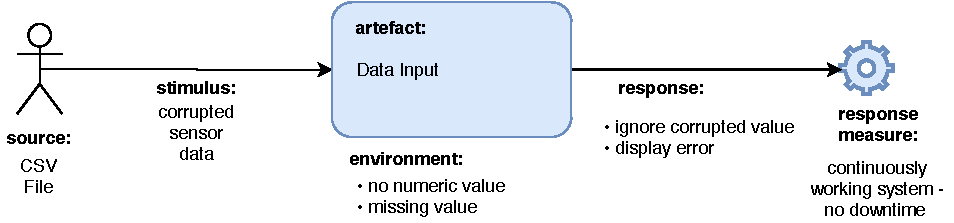
\includegraphics[scale=0.80]{ST_2019_Project_ Requirements/figs/asr_availability.pdf}
    \caption{ASR Availability}
    \label{fig:asr-availability}
\end{figure}

The QAS for the quality attribute \textit{Availability} is triggered by corrupted sensor data inside the CSV file. The error could be caused by a malformed header or non-numeric values. Through a sufficient validation process, misleading values are ignored and the status MISSING will be displayed. This behavior ensures a continuously working system.

\clearpage
\subsection{Functional Completeness}
\label{qa:functionalcompl}
\textbf{ID: QA-\#\ref{qa:functionalcompl}}
\begin{figure}[H]
\centering
    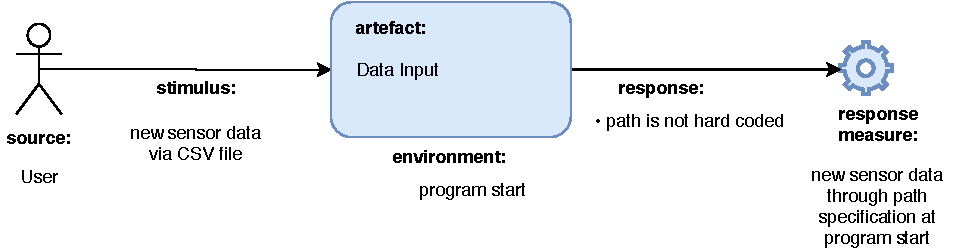
\includegraphics[scale=0.80]{ST_2019_Project_ Requirements/figs/asr_functionalcompl.pdf}
    \caption{ASR Functional Completeness}
    \label{fig:asr-functionalcompl}
\end{figure}

The QAS for the quality attribute \textit{Functional Completeness} is based on the concern of a user to add own sensor data as CSV file. The CSV file selection should be possible through a simple command line argument to allow the usage of any file location.


\clearpage
%%%%
% Specific requirements
%%%%
\section{Specific requirements}
\label{sec:func-req}
\begin{comment}
Actual description of the requirements to a level of detail to enable designers to design a system to satisfy those requirements and testers to test the system. Every requirement should be include the input (stimulus), output (response) and all functions performed by the system. All requirements should be unique! Cross-reference requirements if necessary!

FUNCTIONAL vs. NON-FUNCTIONAL REQUIREMENTS !!!! 

Could be arranged as Use-Case reports / events or as features.
\end{comment}

%\subsection{Requirements Prioritization}
According to Lehtola et al. \cite{b5} and other researches \cite{b6, b7}, requirements prioritization is specified as an informal process and relies highly on individual conditions. To meet the project stakeholders' expectations and keep the project scope along with time constraints in mind, we used the following factors to prioritize the identified requirements in the following order:

\begin{enumerate}
    \item Non-functional requirements (see section \ref{sec:non-func-req})
    \item Project deadline
    \item Cost-value relation
    \item Developer skill level
    \item Technical dept
\end{enumerate}

After an informal discussion between the involved team members and the consideration of the previously mentioned factors, we identified the three priorities a) high, b) medium, and c) low, which are explained in detail in table \ref{table:req-prios}.

\begin{table}[h]
{\renewcommand{\arraystretch}{\arraystrechlength}
    \begin{tabular}{ | >{\columncolor{vu-grey-50}}m{100pt} | m{230pt} | }
    
    \hline
    \rowcolor{vu-blue}
    \textcolor{vu-white}{\textbf{Priority}} & \textcolor{vu-white}{\textbf{Definition}} \\ \hline
    
    High &
    The requirement has to be implemented in all circumstances and has to be delivered with the final release (must have). The actual implementation has to be done exactly as described in this document. Without this requirement, the system does not work.
    \\ \hline
    
    Medium &
    The requirement has to be implemented and has to be delivered with the final release (must have). The requirement does not affect the actual functionality of the system directly. If the actual implementation differs from the requirement specification, the system still works as specified but with less (e.g.) usability.
    \\ \hline
    
    Low &
    The requirement is defined as optional. If all requirements with prioritization high and medium are implemented and the deadline is not yet reached, this requirement could be taken into consideration. Besides, this requirement does not affect the main functionality of the system, but adds upon that.
    \\ \hline
    
    \end{tabular}
}
\caption{Requirements priorities}
\label{table:req-prios}
\end{table}

\clearpage
\subsection{External interface requirements}
\subsubsection{User interfaces}
The command line interface (CLI) is used as an user interface. Therefore all user inputs are received and accepted by the CLI. There is no dedicated graphical user interface. The system feature \textit{User interface} \ref{ftr:ui} examines the user interface in detail.

\subsubsection{Hardware interfaces}
Hardware interface for our application are not directly available, you could however use the CSV to provide captured data from the hardware interface to the application. Which allows external hardware to provide data to our application. This interfacing is limited because it is a playback of readings.

% are required to use the CSV file for communication
\subsubsection{Software interfaces}
% the filesystem
The application uses the software interface for the file system, to read recorded data and write the log if possible to disk.

\subsubsection{Communications interfaces}
% not required or format of the CSV maybe
As communication interface, the program uses the CSV-file format. The exact specifications of this format can be found at \ref{ftr:csv-file}, \ref{ftr:input-recording-location} and an example at \ref{appendix:simulation-csv}.

\clearpage
\subsection{System features}

\begin{comment}
%%%%%%%%%%%%%%%%%%%%%%%%%%%%%%%%%%%%% start example
\subsubsection{Data input - example}
\label{ftr:example}
\renewcommand*{\arraystretch}{1.4}
\begin{longtable}[l]{ | >{\columncolor{vu-grey-50}}m{110pt} | m{300pt} | }

    \hline
    \rowcolor{vu-blue}
    \textcolor{vu-white}{\textbf{Attribute}} & \textcolor{vu-white}{\textbf{Content}}
    \\ \hline
    
    Title &
    example
    \\ \hline
    
    ID &
    SR-\#\ref{ftr:example}
    \\ \hline
    
    Priority &
    High
    \\ \hline
    
    Implemented [in version] &
    yes [1.0]
    \\ \hline
    
    Cross-Reference &
    QA-\#\ref{qa:functionalcompl}
    \\ \hline
    
    Description &
    example
    \\ \hline
    
    Stimulus/Response sequence &
    \begin{itemize}
        \item \textbf{ex}: ex
    \end{itemize}
    \\ \hline
    
    Functional requirements &
    \begin{itemize}
        \item \textbf{FR-\#1}: example
    \end{itemize}
    \\ \hline
\end{longtable}
%%%%%%%%%%%%%%%%%%%%%%%%%%%%%%%%%%%%% end example
\end{comment}

%%%
% Data Input
%%%

%%%%%%%%%%%%%%%%%%%%%%%%%%%%%%%%%%%%% start Input recording location
\subsubsection{Data input - Input recording location}
\label{ftr:input-recording-location}
\renewcommand*{\arraystretch}{1.4}
\begin{longtable}[l]{ | >{\columncolor{vu-grey-50}}m{110pt} | m{300pt} | }

    \hline
    \rowcolor{vu-blue}
    \textcolor{vu-white}{\textbf{Attribute}} & \textcolor{vu-white}{\textbf{Content}}
    \\ \hline
    
    Title &
    Input recording location
    \\ \hline
    
    ID &
    SR-\#\ref{ftr:input-recording-location}
    \\ \hline
    
    Priority &
    High
    \\ \hline
    
    Implemented [in version] &
    Yes [1.0]
    \\ \hline
    
    Cross-Reference &
    QA-\#\ref{qa:functionalcompl}
    \\ \hline
    
    Description &
    The location of the recording should be given to the application as a command-line parameter. This is required to run the application. The format of the recording should be CSV and the first row should be a heading row denoting in which column which value should be.
    \\ \hline
    
    Stimulus/Response sequence &
    \begin{itemize}
        \item \textbf{Argument not given}: Help message should be shown.
        \item \textbf{Argument given}: The  program  should  parse  the  first  line  of  the  argument. This  line  should contain all fields with information of the sensory data. If not, it should show an error message and exit. If there are no errors, the program should continue.
    \end{itemize}
    \\ \hline
    
    Functional requirements &
    \begin{itemize}
        \item \textbf{FR-\#1}: The location of the recording should be given by a command-line argument, \textit{-}\textit{-path}.
        \item \textbf{FR-\#2}: The recording should be written in CSV format using "," (comma) as a separator. (see SR-\#\ref{ftr:csv-file})
        \item \textbf{FR-\#3}: Incomplete or incorrect header information will result in showing the same help information as missing \textit{-}\textit{-path}, with information showing how to point to a correct CSV.
    \end{itemize}
    \\ \hline
\end{longtable}
%%%%%%%%%%%%%%%%%%%%%%%%%%%%%%%%%%%%% end Input recording location


%%%%%%%%%%%%%%%%%%%%%%%%%%%%%%%%%%%%% start CSV file

\clearpage
\subsubsection{Data input - CSV file}
\label{sec:data-input:csv-file}
\label{ftr:csv-file}
\renewcommand*{\arraystretch}{1.4}
\begin{longtable}[l]{ | >{\columncolor{vu-grey-50}}m{110pt} | m{300pt} | }

    \hline
    \rowcolor{vu-blue}
    \textcolor{vu-white}{\textbf{Attribute}} & \textcolor{vu-white}{\textbf{Content}}
    \\ \hline
    
    Title &
    Comma-separated values (CSV) file
    \\ \hline
    
    ID &
    SR-\#\ref{ftr:csv-file}
    \\ \hline
    
    Priority &
    High
    \\ \hline
    
    Implemented [in version] &
    Yes [1.0]
    \\ \hline
    
    Cross-Reference &
    QA-\#\ref{qa:functionalcompl}; SR-\#\ref{ftr:input-recording-location}; SR-\#\ref{ftr:ui}
    \\ \hline
    
    Description &
    The  system  collects  the  data  from  a  CSV  file  exclusively  which  simulates  real  sensor  data. The CSV file is given as command line argument at program start. The file will also be used to simulate broken-, corrupted- or defect-sensors.
    \\ \hline
    
    Stimulus/Response sequence &
    \begin{itemize}
        \item \textbf{CSV file is given}: The program starts as excepted and starts reading from file and starts with data processing.
        \item \textbf{CSV file is NOT given}: The program provides the help message.
        \item \textbf{CSV file is given but does not exists}: The program provides the help message.
        \item \textbf{CSV file contains a corrupted header}: The program provides the help message.
        \item \textbf{CSV file contains corrupted data/values}: The program starts and reads from file. If the values are out of range (see processor for detailed ranges) the value will be counted as 0 and MISSING (see SR-\#\ref{ftr:ui}).
        \item \textbf{Not enough rights to read the file}: The program does not have enough rights to read the file, the program should show the help message and exit.
    \end{itemize}
    \\ \hline
    
    Functional requirements &
    \begin{itemize}
        \item \textbf{FR-\#1}: The recording should be written in CSV format according \textbf{rfc4180} \cite{rfc4180}.
        \item \textbf{FR-\#2}: The CSV format should be using "," (comma) as a separator.
        \item \textbf{FR-\#3}: The CSV format should be able to handle line endings in Windows (CRLF), Linux (LF) and MacOS (LF) format.
        \item \textbf{FR-\#4}: The first row of the CSV is a heading row, containing all of the following values in any order: \textit{oxygen,pulse,blood\_pressure\_systolic,blood\_pressure\_diastolic}. These values denote the order of the columns, and are used by the program to determine which column has which data so it can parse it correctly.
        \item \textbf{FR-\#5}: Every row in the CSV file represents one second of recording.
    \end{itemize}
    \\ \hline
    
    Example &
    An example CSV file listing can be found in appendix \ref{appendix:simulation-csv}
    \\ \hline
\end{longtable}
%%%%%%%%%%%%%%%%%%%%%%%%%%%%%%%%%%%%% end CSV file


%%%
% Data Processing
%%%

%%%%%%%%%%%%%%%%%%%%%%%%%%%%%%%%%%%%% start oxygen measurements
\clearpage
\subsubsection{Data processing - Oxygen measurements}
\label{ftr:oxygen}
\renewcommand*{\arraystretch}{1.4}
\begin{longtable}[l]{ | >{\columncolor{vu-grey-50}}m{110pt} | m{300pt} | }

    \hline
    \rowcolor{vu-blue}
    \textcolor{vu-white}{\textbf{Attribute}} & \textcolor{vu-white}{\textbf{Content}}
    \\ \hline
    
    Title &
    Oxygen measurements
    \\ \hline
    
    ID &
    SR-\#\ref{ftr:oxygen}
    \\ \hline
    
    Priority &
    High
    \\ \hline
    
    Implemented [in version] &
    Yes [1.0]
    \\ \hline
    
    Cross-Reference &
    QA-\#\ref{qa:reliability}; SR-\#\ref{ftr:ui}
    \\ \hline
    
    Description &
    The heartbeat monitor needs to sensor multiple measurements. One of them is oxygen. When an oxygen measurement comes in, it needs to be checked if the oxygen saturation levels are correct in the blood.
    \\ \hline
    
    Stimulus/Response sequence &
    \begin{itemize}
        \item \textbf{Incoming measurement}: The measurement is processed by a processor, which analyses the value and returns the right status message.
        % \item \textbf{Measurement value is normal}: Process measurement.
        % \item \textbf{Measurement value is abnormal}: Trigger alarm.
    \end{itemize}
    \\ \hline
    
    Functional requirements &
    \begin{itemize}
        \item \textbf{FR-\#1}: Return correct status message for the current oxygen level. The correct messages are: 
            \begin{itemize}
                \item OK for oxygen 95 or higher
                \item MINOR for oxygen 90 to 94 (inclusive)
                \item MAJOR for oxygen 61 to 89 (inclusive)
                \item LIFE\_THREATENING for oxygen 60 or below
            \end{itemize}
        \item \textbf{FR-\#2}: Return MISSING status message when the value for oxygen is not a number or outside the range of 0 and 100 (numbers are inclusive).
        \item \textbf{FR-\#3}: The statistics of each value should be kept track of.
        \item \textbf{FR-\#4}: Values can only be positive integers.
    \end{itemize}
    \\ \hline
    
    References &
    Oxygen stages: \cite{b9}
    \\ \hline
\end{longtable}
%%%%%%%%%%%%%%%%%%%%%%%%%%%%%%%%%%%%% end oxygen


%%%%%%%%%%%%%%%%%%%%%%%%%%%%%%%%%%%%% start pulse measurements

\clearpage
\subsubsection{Data processing - Pulse measurements}
\label{ftr:pulse}
\renewcommand*{\arraystretch}{1.4}
\begin{longtable}[l]{ | >{\columncolor{vu-grey-50}}m{110pt} | m{300pt} | }

    \hline
    \rowcolor{vu-blue}
    \textcolor{vu-white}{\textbf{Attribute}} & \textcolor{vu-white}{\textbf{Content}}
    \\ \hline
    
    Title &
    Pulse measurements
    \\ \hline
    
    ID &
    SR-\#\ref{ftr:pulse}
    \\ \hline
    
    Priority &
    High
    \\ \hline
    
    Implemented [in version] &
    Yes [1.0]
    \\ \hline
    
    Cross-Reference &
    QA-\#\ref{qa:reliability}; SR-\#\ref{ftr:ui}
    \\ \hline
    
    Description &
    The heartbeat monitor needs to sensor multiple measurements.  One of them is pulse.  When the measurement comes in it needs to be checked if it is a valid measurement and in which category the measurement falls.
    \\ \hline
    
    Stimulus/Response sequence &
    \begin{itemize}
        \item \textbf{Incoming measurement}: The measurement is processed by a processor, which analyses the value and returns the right status message.
        % \item \textbf{Measurement value is normal}: Process measurement.
        % \item \textbf{Measurement value is abnormal}: Trigger alarm.
    \end{itemize}
    \\ \hline
    
    Functional requirements &
    \begin{itemize}
        \item \textbf{FR-\#1}: Return the correct status messages for the current pulse. The correct message are, numbers are inclusive:
            \begin{itemize}
                \item Min pulse 60, max pulse 100 = OK
                \item Min pulse 50, max pulse 120 = MINOR
                \item Min pulse 40, max pulse 160 = MAJOR
                \item Min pulse 1, max pulse 230 = LIFE\_THREATENING
                \item Any other values should be considered MISSING
            \end{itemize}
        \item \textbf{FR-\#2}: The statistics of each value should be kept track of.
        \item \textbf{FR-\#3}: Values can only be positive integers.
    \end{itemize}
    \\ \hline
    
    References &
    \begin{itemize}
        \item Minimum heart rate: \cite{resting-heart-rate}
        \item After the age of 10, 60 to 100 is considered normal in a resting position (not including factors such as stress and exercise etc...) \cite{target-training-heart-rates, target-heart-rates}
    \end{itemize}
    \\ \hline
    
\end{longtable}
%%%%%%%%%%%%%%%%%%%%%%%%%%%%%%%%%%%%% end pulse



%%%%%%%%%%%%%%%%%%%%%%%%%%%%%%%%%%%%% start pulse measurements

\clearpage
\subsubsection{Data processing - Blood pressure measurements}
\label{ftr:bloodpressure}
\renewcommand*{\arraystretch}{1.4}
\begin{longtable}[l]{ | >{\columncolor{vu-grey-50}}m{110pt} | m{300pt} | }

    \hline
    \rowcolor{vu-blue}
    \textcolor{vu-white}{\textbf{Attribute}} & \textcolor{vu-white}{\textbf{Content}}
    \\ \hline
    
    Title &
    Blood pressure measurements
    \\ \hline
    
    ID &
    SR-\#\ref{ftr:bloodpressure}
    \\ \hline
    
    Priority &
    High
    \\ \hline
    
    Implemented [in version] &
    yes [1.0]
    \\ \hline
    
    Cross-Reference &
    QA-\#\ref{qa:reliability}; SR-\#\ref{ftr:ui}
    \\ \hline
    
    Description &
    The heartbeat monitor needs to sensor multiple measurements. One of them is blood pressure.  When the measurement comes in it needs to be checked if it is a valid measurement and in which category the measurement falls.
    \\ \hline
    
    Stimulus/Response sequence &
    \begin{itemize}
        \item \textbf{Incoming measurement}: The two measurement values diastolic and systolic are processed by a processor, which analyses the value and returns the right status message.
    \end{itemize}
    \\ \hline
    
    Functional requirements &
    \begin{itemize}
        \item \textbf{FR-\#1}: Return the correct status messages for the current \textbf{diastolic} blood pressure. Numbers are inclusive:
        \begin{itemize}
            \item higher then or equal to 120 = LIFE\_THREATENING
            \item lower then 40 = LIFE\_THREATENING
            \item higher then or equal to 90 = MAJOR
            \item lower then 50 = MAJOR
            \item higher then or equal to 80 = MINOR
            \item lower then 60 = MINOR
            \item between 60 (inclusive) and 79 (inclusive) = OK
            \item values cannot be parsed, or are missing = MISSING.
        \end{itemize}
    \end{itemize}
    \\ \hline
\end{longtable}

\clearpage
\begin{longtable}[l]{ | >{\columncolor{vu-grey-50}}m{110pt} | m{300pt} | }
    \hline
    Functional requirements &
    \begin{itemize}
    % systolic
    % diastolic
        \item \textbf{FR-\#2}: Return the correct status messages for the current \textbf{systolic} blood pressure. Numbers are inclusive:
            \begin{itemize}
                \item higher then or equal to 180 = LIFE\_THREATENING
                \item lower then 40 = LIFE\_THREATENING
                \item higher then or equal to 140 = MAJOR
                \item lower then 60 = MAJOR
                \item higher then or equal to 130 = MINOR
                \item lower then 90 = MINOR
                \item between 90 (inclusive) and 129 (inclusive) = OK
                \item value that cannot be parsed, or are missing = MISSING.

            \end{itemize}
        \item \textbf{FR-\#3}: The statistics of each value should be kept track of.
        \item \textbf{FR-\#4}: Values can only be positive integers.
    \end{itemize}
    \\ \hline
    
    References &
    Blood pressure stages: \cite{b8}
    \\ \hline
    
\end{longtable}
%%%%%%%%%%%%%%%%%%%%%%%%%%%%%%%%%%%%% end blood pressure






%%%%%%%%%%%%%%%%%%%%%%%%%%%%%%%%%%%%% start user interface
%%%%%%%%%%%%%%%%%%%%%%%%%%%%%%%%%%%%% start Statistic

\clearpage
\subsubsection{Data output - Statistic}
\label{ftr:statistic}
\renewcommand*{\arraystretch}{1.4}
\begin{longtable}[l]{ | >{\columncolor{vu-grey-50}}m{110pt} | m{300pt} | }

    \hline
    \rowcolor{vu-blue}
    \textcolor{vu-white}{\textbf{Attribute}} & \textcolor{vu-white}{\textbf{Content}}
    \\ \hline
    
    Title &
    Data output - statistic
    \\ \hline
    
    ID &
    SR-\#\ref{ftr:statistic}
    \\ \hline
    
    Priority &
    Medium
    \\ \hline
    
    Implemented [in version] &
    Yes [1.0]
    \\ \hline
    
    Cross-Reference &
    SR-\#\ref{ftr:ui}; SR-\#\ref{ftr:oxygen}; SR-\#\ref{ftr:pulse}; SR-\#\ref{ftr:bloodpressure}
    \\ \hline
    
    Description &
        After running the simulation a statistics overview is given of each measurement and how often they occurred. Beyond, the total number of recordings should be shown (up until that point).
    \\ \hline
    
    Stimulus/Response sequence &
    \begin{itemize}
        \item \textbf{Just before the program ends}: If all data rows are processed, the statistics should be shown.
    \end{itemize}
    \\ \hline
    
    Functional requirements &
    \begin{itemize}
        \item \textbf{FR-\#1}: The statistics for pulse, oxygen, blood pressure systolic and blood pressure diastolic should be shown.
        \item \textbf{FR-\#2}: When a statistics is shown it shows the number of OK, MISSING, MINOR, MAJOR, and LIFE\_THREATENING measurement values.
        \item \textbf{FR-\#3}: It shows the number of processed measurements.
    \end{itemize}
    \\ \hline
    
\end{longtable}
%%%%%%%%%%%%%%%%%%%%%%%%%%%%%%%%%%%%% end Statistic

%%%
% Data Output
%%%


\clearpage
\subsubsection{Data output - User interface}
\label{ftr:ui}
\renewcommand*{\arraystretch}{1.4}
\begin{longtable}[l]{ | >{\columncolor{vu-grey-50}}m{110pt} | m{300pt} | }

    \hline
    \rowcolor{vu-blue}
    \textcolor{vu-white}{\textbf{Attribute}} & \textcolor{vu-white}{\textbf{Content}}
    \\ \hline
    
    Title &
    User interface
    \\ \hline
    
    ID &
    SR-\#\ref{ftr:ui}
    \\ \hline
    
    Priority &
    Medium
    \\ \hline
    
    Implemented [in version] &
    yes [1.0]
    \\ \hline
    
    Cross-Reference &
    QA-\#\ref{qa:functionalcompl}; QA-\#\ref{qa:reliability}
    \\ \hline
    
    Description &
    The user interface provides arguments at program start. After this phase the system doesn't take any other input. While the program is running, the interface will update the user with a constant flow of messages at the interval defined in \ref{sec:data-input:csv-file} FR-\#5. The messages will contain information according to table \ref{table:output_format}.
    
    The status of a particular value (Pulse, Oxygen saturation, Systolic, Diastolic) is one of: OK, MISSING, MINOR, MAJOR, LIFE\_THREATENING which is generated according to the processing of the system. These values are explained in table \ref{table:color_format}.
    \\ \hline
    
    Stimulus/Response sequence &
    \begin{itemize}
        \item \textbf{Measurement-Result ready to present}: If there are more results to display, the system will output these results as soon as they are ready in the order they are coming in (FIFO).
        \item \textbf{No Measurement-Result ready to present}: If there are no more results to display, the system will output statistics after which the system will shutdown.
    \end{itemize}
    \\ \hline
    
    Functional requirements &
    \begin{itemize}
        \item \textbf{FR-\#1}: All status messages will have a timestamp.
        \item \textbf{FR-\#2}: Status message should contain the status of oxygen, pulse,  blood\_pressure\_systolic and blood\_pressure\_diastolic.
        \item \textbf{FR-\#3}: Status message should contain the value of oxygen, pulse,  blood\_pressure\_systolic and blood\_pressure\_diastolic.
        \item \textbf{FR-\#4}: Status message should appear on a constant level. At the end of the program it should show the statistics of the monitoring.
    \end{itemize}
    \\ \hline
\end{longtable}

\begin{table}[H]
{\renewcommand{\arraystretch}{\arraystrechlength}
    \begin{tabular}{ | >{\columncolor{vu-grey-50}}m{95pt} | m{100pt} | m{170pt} | }
    
    \hline
    \rowcolor{vu-blue}
    \textcolor{vu-white}{\textbf{Line}} & 
    \textcolor{vu-white}{\textbf{Format}} & 
    \textcolor{vu-white}{\textbf{Elaboration}} \\ \hline
    
    Timestamp &
    \texttt{[dd-mm-yy HH:MM:SS]} &
    The time in the format d-m-y H:M:S (little-endian) according to Dutch standards with a 24 hour clock according to ISO 8601.
    \\ \hline
    
    Pulse &
    \texttt{Pulse: 000 bpm} &
    The pulse of the patient in BPM
    \\ \hline
    
    Pulse Status &
    \texttt{status: STATUS} &
    The status of the pulse sensor according to the simulation.
    \\ \hline
    
    Oxygen saturation &
    \texttt{SaO2: 000\%} &
    The oxygen saturation of the patient in SaO2 percentage.
    \\ \hline
    
    Oxygen Status &
    \texttt{status: STATUS} &
    The status of the oxygen sensor according to the simulation.
    \\ \hline
    
    Blood pressure &
    \texttt{Blood pressure: 0/0 mm Hg} &
    The blood pressure of the patient in systolic over diastolic mm Hg.
    \\ \hline
    
    Systolic Status &
    \texttt{status: STATUS} &
    The status of the systolic sensor according to the simulation.
    \\ \hline
    
    Diastolic Status &
    \texttt{status: STATUS} &
    The status of the diastolic sensor according to the simulation.
    \\ \hline
    
    \end{tabular}
}
\caption{The values required in the output}
\label{table:output_format}
\end{table}

\begin{table}[H]
{\renewcommand{\arraystretch}{\arraystrechlength}
    \begin{tabular}{ | >{\columncolor{vu-grey-50}}m{105pt} | m{200pt} | }
    
    \hline
    \rowcolor{vu-blue}
    \textcolor{vu-white}{\textbf{Status}} &
    \textcolor{vu-white}{\textbf{Elaboration}}
    \\ \hline
    
    OK &
    A reading that is not considered dangerous
    \\ \hline
    MISSING &
    Missing indicates any value that cannot be considered a valid value from the sensor. This includes, readings that are too high, too low, missing or of incorrect format.
    \\ \hline
    MINOR &
    A reading that is of interest to medical personnel but cannot be considered a threat yet.
    \\ \hline
    MAJOR &
    A reading that is of interest to medical personnel and has to be considered a threat.
    \\ \hline
    LIFE\_THREATENING &
    A reading that is of interest to medical personnel because it can have severe effects on the chance of survival of the patient.
    \\ \hline
    \end{tabular}
}
\caption{Notification Levels}
\label{table:color_format}
\end{table}
%%%%%%%%%%%%%%%%%%%%%%%%%%%%%%%%%%%%% end user interface
%%%%%%%%%%%%%%%%%%%%%%%%%%%%%%%%%%%%% start logging
\clearpage
\subsubsection{Data output - Logging}
\label{ftr:logging}
\renewcommand*{\arraystretch}{1.4}
\begin{longtable}[l]{ | >{\columncolor{vu-grey-50}}m{110pt} | m{300pt} | }

    \hline
    \rowcolor{vu-blue}
    \textcolor{vu-white}{\textbf{Attribute}} & \textcolor{vu-white}{\textbf{Content}}
    \\ \hline
    
    Title &
    Logging
    \\ \hline
    
    ID &
    SR-\#\ref{ftr:logging}
    \\ \hline
    
    Priority &
    Low
    \\ \hline
    
    Implemented [in version] &
    yes [1.0]
    \\ \hline
    
    Cross-Reference &
    SR-\#\ref{ftr:ui}
    \\ \hline
    
    Description &
    The system puts every status and statistic that is to be printed on the screen in a file. The filename will change according to the date. The files will be stored in the module folder logs. If the system cannot log due to lack of space or lack of rights for writing in the location, it will provide a message.
    \\ \hline
    
    Stimulus/Response sequence &
    \begin{itemize}
        \item \textbf{New result to log without log folder}: If a new result is ready the logger will try to log this and create a new log folder with a new log file to parse the logs in.
        \item \textbf{New result to log with log folder with existing log file}: If a new result is ready the logger will try to log this an create a new log in the existing folder and append to the existing log file that corresponds to the current date.
        \item \textbf{New result to log with log folder without existing log file}:  If a new result is ready the logger will try to log this an create a new log in the existing folder and create a new log file according to the current date.
        \item \textbf{New result to log without writing access}: If a new result is ready the logger will try to log this. If it fails due to insufficient access rights, the system will update the user about this and no logging will be available for the session until the user gets access to write in the folder.
        \item \textbf{New result to log with no space left}: If a new result is ready the logger will try to log this. If it fails due to insufficient space, the system will update the user about this and no logging will be available for the session until the user makes space for logs.
    \end{itemize}
    \\ \hline
    
    Functional requirements &
    \begin{itemize}
        \item \textbf{FR-\#1}: The logger should create a log for every status message and statistic.
        \item \textbf{FR-\#2}: The logger should create a logfile for the current date if it does not exist
        \item \textbf{FR-\#3}: The logger should append to the logfile for the current date if it does exist
        \item \textbf{FR-\#4}: The logger should create a log folder if this folder does not exist
        \item \textbf{FR-\#5}: The logger should show a single message if it cannot log due to lack of space
        \item \textbf{FR-\#6}: The logger should show a single message if it cannot log due to lack of access rights
        
    \end{itemize}
    \\ \hline
    
\end{longtable}
%%%%%%%%%%%%%%%%%%%%%%%%%%%%%%%%%%%%% end logging

\clearpage
\subsection{Performance requirements}
No performance requirements are specified since the system adhere rather to a sequential process than a parallel or time critical process.

\subsection{Other requirements}
\subsubsection{Python Version}
The system shall be developed with the Python version 3.7.7. Used and recommended Python packages and libraries are specified in appendix \ref{appendix:python-libs}.


\subsubsection{Code Style-guide}
The code development shall adhere to the "PEP 8 -- Style Guide for Python Code"\footnote{https://www.python.org/dev/peps/pep-0008/} and shall be fulfilled by using the Python code formatter \textit{Black}\footnote{https://github.com/psf/black} (version 19.10b0).

\subsubsection{Usage}
\subsubsection*{System start}
\begin{itemize}
    \item The system executable should only be opened via a terminal (Windows, Unix, MacOS see section \ref{sec:constraints}).
    \item \textbf{Opening the executable via double-click or any other way is \textit{not} supported.}
\item Step-by-Step: \begin{enumerate}
    \item Preconditions:
        \begin{enumerate}
            \item Make sure you have the correct executable for your platform \texttt{HB-Sim2020.exe} (Windows filename) or \texttt{HB-Sim2020} (Linux and MacOS filename).
            \item Make sure the executable and \texttt{simulations.csv} are in the same folder.
            \item Make sure the executable has executable rights on MacOS and Linux.
            \item For logging the folder the executable resides in needs to have write permissions and enough free space, this is the case for all platforms. If the program does not have write permissions it will still run but give a message about it and not generate any logs files.
        \end{enumerate}
    \item Open a command-line interface
    \item Go to the folder holding both files
    \item Run (Windows): \texttt{./HB-Sim2020.exe --path simulation.csv}
    \item Run (Unix): \texttt{./HB-Sim2020 --path simulation.csv}
    \item Run (MacOS): \texttt{./HB-Sim2020 --path simulation.csv}
\end{enumerate}
\end{itemize}

\subsubsection*{System termination}
The system is terminated/ends in two different ways:
\begin{itemize}
    \item System reaches the end of the CSV. There are no more measurements to process. The program will be end automatically.
    \item The user can terminate the program at any time by pressing \texttt{ctrl + c}
\end{itemize}


\subsubsection{Python Executable}
The releases are created with the Python library \textit{PyInstaller}\footnote{https://pypi.org/project/PyInstaller/} (version 3.6) to create executables for Windows, Unix, and MacOS. Every release should be packed as ZIP and contain the executable itself and one CSV-file with simulation data.
\subsubsection*{Known Bug}
PyInstaller itself contains of a known bug (see \footnote{https://github.com/pyinstaller/pyinstaller/issues/2349} and \footnote{https://github.com/pyinstaller/pyinstaller/issues/3646}) by handling \texttt{KeyboardInterrups}. Due to this issue, it could be that the program terminates with an exception while pressing \texttt{ctrl + c}, for instance \texttt{Failed to execute script heartbeatmonitor}. Since this is a known issue, this should be taken into account for next releases.

\clearpage
%%%%
% Appendix
%%%%
\section{Appendix}
\subsection{Used Python Libraries}
\label{appendix:python-libs}
\begin{table}[h]
{\renewcommand{\arraystretch}{\arraystrechlength}
    \begin{tabular}{ | m{100pt} | m{230pt} | }
    
    \hline
    \rowcolor{vu-blue}
    \textcolor{vu-white}{\textbf{Library}} & \textcolor{vu-white}{\textbf{Notes}} \\ \hline
    
    \texttt{Python} &
    Version 3.7.7
    \\ \hline
    
    \texttt{os} &
    Os is used for making sure a file or folder does (not) exist, creating the paths to files and folders with the correct separators depending on your system, making directories, to get the line separator for this operating system/platform.
    \\ \hline
    
    \texttt{sys} &
    Sys is used for getting the command-line arguments, and setting the exit code for the program.
    \\ \hline
    
    \texttt{typing} &
    Typing is used for type hinting with denoting build-in types as Dict and List.
    \\ \hline
    
    \texttt{datetime} &
    Used for getting the current date and time and formatting it correctly for human display.
    \\ \hline
    
    \texttt{csv} &
    Is used for reading from a CSV file.
    \\ \hline
    
    \texttt{time} &
    Used for making the program "sleep"/wait for a certain time and so simulating that we're waiting on new sensor readings.
    \\ \hline
    
    \texttt{errno} &
    Used for determining the error when wanting to write a file to disk and something went wrong.
    \\ \hline
    
    \texttt{pathlib} &
    Used for getting to the parent directory, in a file path string.
    \\ \hline
    
    \texttt{enum} &
    Used for making enum objects in the code.
    \\ \hline
    
    \end{tabular}
}
\end{table}

\clearpage
\subsection{Simulation Data - CSV}
\label{appendix:simulation-csv}
\begin{lstlisting}[caption=CSV example, captionpos=b]
oxygen,pulse,blood_pressure_systolic,blood_pressure_diastolic
95,80,100,70
96,87,101,74
94,85,101,75
95,83,101,74
97,85,102,72
94,89,103,68
94,88,104,64
93,82,105,62
94,75,106,60
93,73,106,59
92,70,105,60
90,68,108,55
90,67,109,54
85,65,110,52
86,63,118,49
85,61,115,47
86,59,116,46
84,57,120,42
85,53,121,38
\end{lstlisting}





\clearpage
%%%%
% Example Tables
%%%%
\begin{comment}
\section{Tables}
All tables are colored by the VU corporate identity colors. See preamble section \texttt{VU colors}.

\subsection{Example \#1}
\begin{table}[h]
{\renewcommand{\arraystretch}{\arraystrechlength}
    \begin{tabular}{ | >{\columncolor{vu-grey-50}}m{100pt} | m{230pt} | }
    
    \hline
    \rowcolor{vu-blue}
    \textcolor{vu-white}{\textbf{Headline 1}} & \textcolor{vu-white}{\textbf{Headline 2}} \\ \hline
    
    Example &
    My cell example
    \\ \hline
    
    Example &
    Lorem ipsum
    \\ \hline
    
    \end{tabular}
}
\end{table}


\subsection{Example \#2}
\begin{table}[h]
{\renewcommand{\arraystretch}{\arraystrechlength}
    \begin{tabular}{ | >{\columncolor{vu-blue}\color{vu-white}}m{100pt} | m{230pt} | }
    \hline
    
    \textbf{Example} &
    Lorem ipsum
    \\ \hline
    
    \textbf{Example} &
    Lorem ipsum
    \\ \hline
    
    \textbf{Example} &
    Lorem ipsum
    \\ \hline
    
    \end{tabular}
}
\end{table}


\subsection{Example \#3}
\begin{table}[h]
{\renewcommand{\arraystretch}{\arraystrechlength}
\begin{tabular}{ | >{\columncolor{vu-blue}\color{vu-white}}m{70pt} | >{\columncolor{vu-grey-50}}m{330pt} | } 
\hline
Example                  & \textbf{Con\#1}: Example \\ 
\hline
Example         & \makecell*[l]{\textbf{Cr\#1}: Example \\ \textbf{Cr\#2}: Example}  \\
\hline
\end{tabular}
}
\end{table}


\subsection{Example \#4}
\begin{table}[H]
{\renewcommand{\arraystretch}{\arraystrechlength}
\begin{tabular}{ | >{\columncolor{vu-blue}\color{vu-white}}m{70pt} | >{\columncolor{vu-grey-50}}m{80pt} | p{238pt} | } 
\hline
Option 1                  & Example & \textbf{Example}: Lorem Ipsum  \\ 
\hline
                          & Example   & Lorem ipsum dolor sit amet, consetetur sadipscing elitr, sed diam nonumy eirmod tempor invidunt ut labore et dolore magna aliquyam erat, sed diam voluptua. At vero eos et accusam et justo duo dolores et ea rebum. Stet clita kasd gu                   \\ 
\hline
                          & Example  & Example.                        \\ 
\hline
                          & Example  & \makecell*[{{p{238pt}}}]{
                          Lorem \\ \\
                          Ipsum
                          }\\ 

\hline
\end{tabular}
}
\end{table}
\end{comment}



\clearpage
\begin{thebibliography}{00}
\bibitem{b1}World Health Organization, \textit{Pulse Oximetry Training Manual}, World Heal. Organ., pp. 1–23, 2011.
\bibitem{b2}Wikipedia contributors, \textit{Heart rate}, Wikipedia, The Free Encyclopedia, https://en.wikipedia.org/w/index.php?title=Heart\_rate&oldid=952483498 (accessed April 23, 2020).
\bibitem{b3}Wikipedia contributors, \textit{Oxygen saturation (medicine)}, Wikipedia, The Free Encyclopedia, https://en.wikipedia.org/w/index.php?title=Oxygen\_saturation\_(medicine)&oldid=952492535 (accessed April 23, 2020).
\bibitem{b4}Wikipedia contributors, \textit{Blood pressure}, Wikipedia, The Free Encyclopedia, https://en.wikipedia.org/w/index.php?title=Blood\_pressure&oldid=951946682 (accessed April 23, 2020).
\bibitem{b5}L. Lehtola, M. Kauppinen, and S. Kujala, \textit{Requirements Prioritization Challenges in Practice}, in Lecture Notes in Computer Science (including subseries Lecture Notes in Artificial Intelligence and Lecture Notes in Bioinformatics), vol. 3009, no. April, 2004, pp. 497–508.
\bibitem{b6}A. S. I. Mohamed, B. I. A. El-Maddah, and C. A. M. Wahba, \textit{Criteria-based requirements prioritization for software product management}, Proc. 2008 Int. Conf. Softw. Eng. Res. Pract. SERP 2008, no. January, pp. 587–593, 2008.
\bibitem{b7}J. Karlsson and K. Ryan, \textit{A cost-value approach for prioritizing requirements}, IEEE Softw., vol. 14, no. 5, pp. 67–74, 1997.
\bibitem{b8}T. Kirkpatrick and K. Tobias, \textit{Health System PEDIATRIC AGE SPECIFIC Self Learning Module}, pp. 1–11, 2009.
\bibitem{rfc4180}]Y. Shafranovich, \textit{RFC 4180 - Common Format and MIME Type for CSV Files}, iet.org, 2005. [Online]. Available: https://www.ietf.org/rfc/rfc4180.txt. [Accessed: 25-Apr-2020].
\bibitem{b9}Abdo, Wilson F, and Leo M A Heunks. \textit{Oxygen-induced hypercapnia in COPD: myths and facts.} Critical care (London, England) vol. 16,5 323. 29 Oct. 2012, doi:10.1186/cc11475
\bibitem{resting-heart-rate}https://thenextchallenge.org/resting-heart-rate/
\bibitem{target-training-heart-rates}https://www.medicalnewstoday.com/articles/235710#target-training-heart-rates
\bibitem{target-heart-rates}https://www.heart.org/en/healthy-living/fitness/fitness-basics/target-heart-rates
\end{thebibliography}



\end{document}
